\documentclass{article}
\usepackage[T1]{fontenc}
\usepackage{graphicx}
\usepackage{enumitem}
\usepackage{float}
\usepackage{fancyhdr}
\pagestyle{fancy}
\usepackage{hyperref}
\graphicspath{{Slike/}}
\fancyhf{}





\title{Konfiguracija Osobnog Računala}
\author{Dominik Jurusic}
\date{\today}

\begin{document}

\maketitle
\tableofcontents
\listoffigures
\pagebreak



\section{Svrha Računala}
Svrha računala je bila 

\section{Komponente}

\subsection{Procesor (CPU)}
\begin{figure}[H]
    \centering
    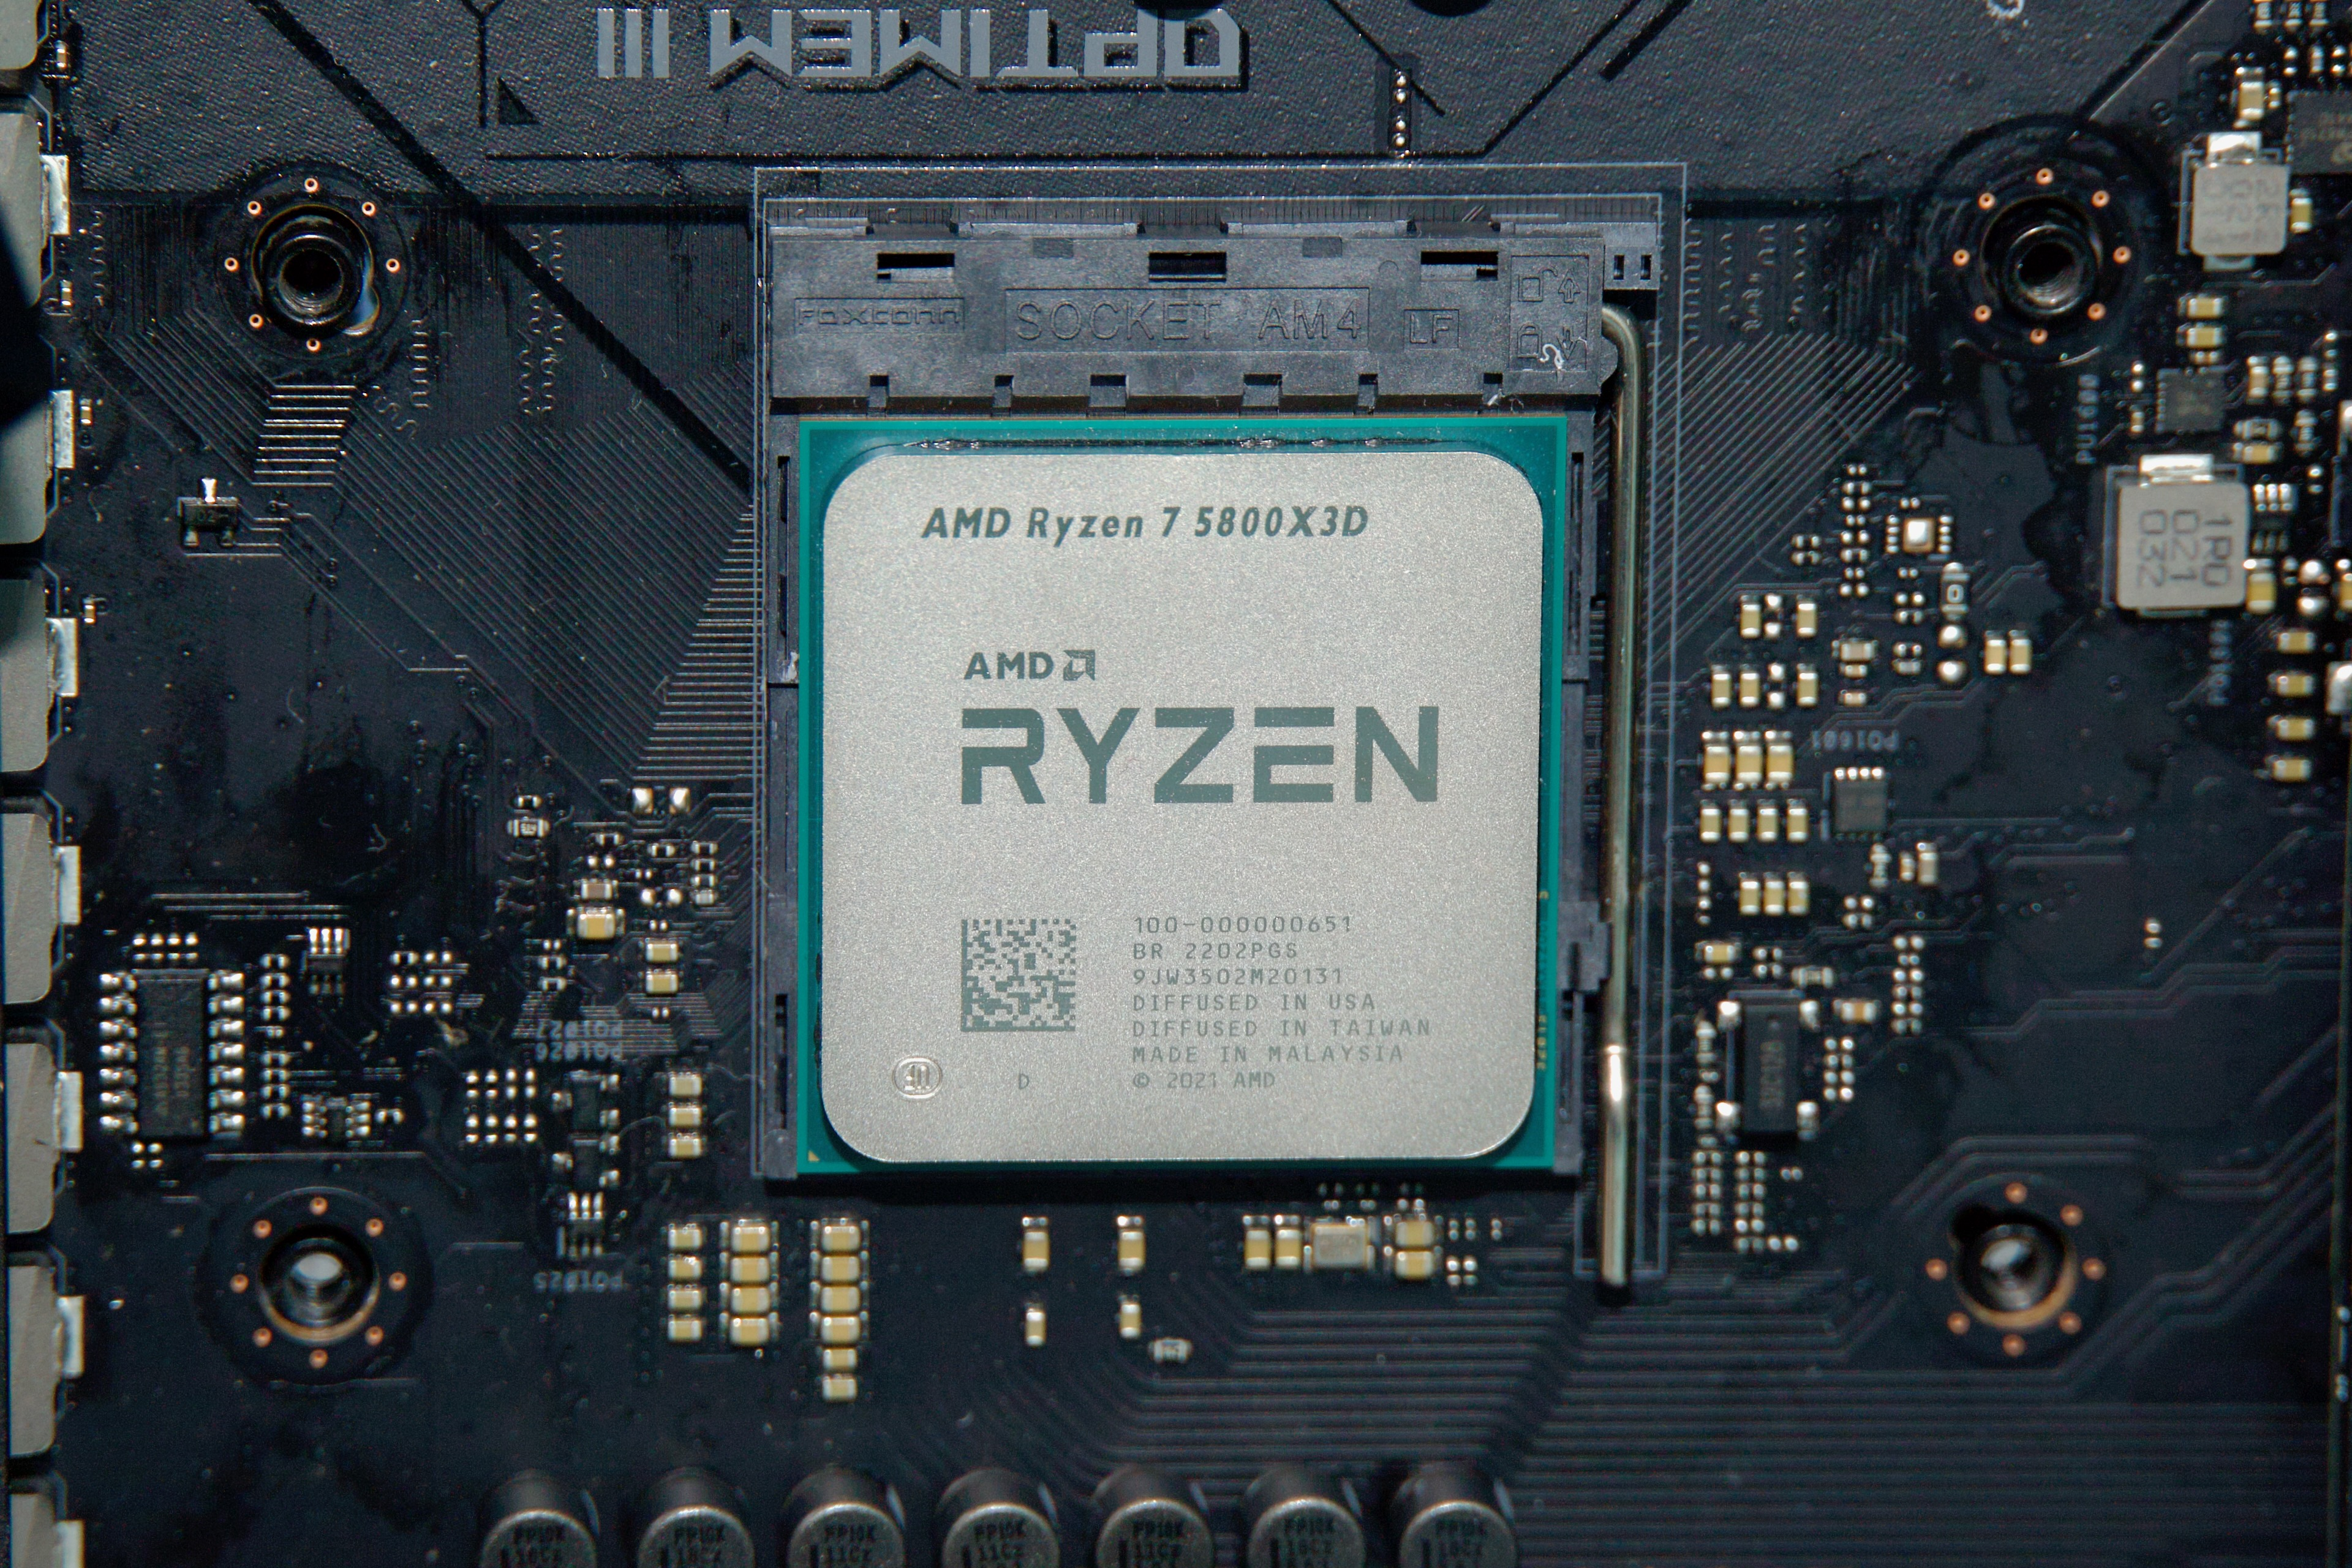
\includegraphics[scale=0.1]{Slike/CPU.jpg}
    \caption{AMD Ryzen 7 5800X3D}
    \label{fig:Procesor}
\end{figure}
\begin{itemize}
    \item Model: Ryzen 7 5800x3d
    \item Brzina: 3.4 GHz (base), 4.5 GHz (boost)
    \item Broj jezgara: 8, Broj dretvi: 16
    \item Obrazloženje: Odabran zbog visokih performansi 
    \item Cijena: 370 EUR (\href{https://www.adm.hr/cpu-amd-ryzen-7-5800x3d-box-am4-100-100000651wof/72892/product/}{Shop})
\end{itemize}

\subsection{Grafička kartica}
\begin{figure}[H]
    \centering
    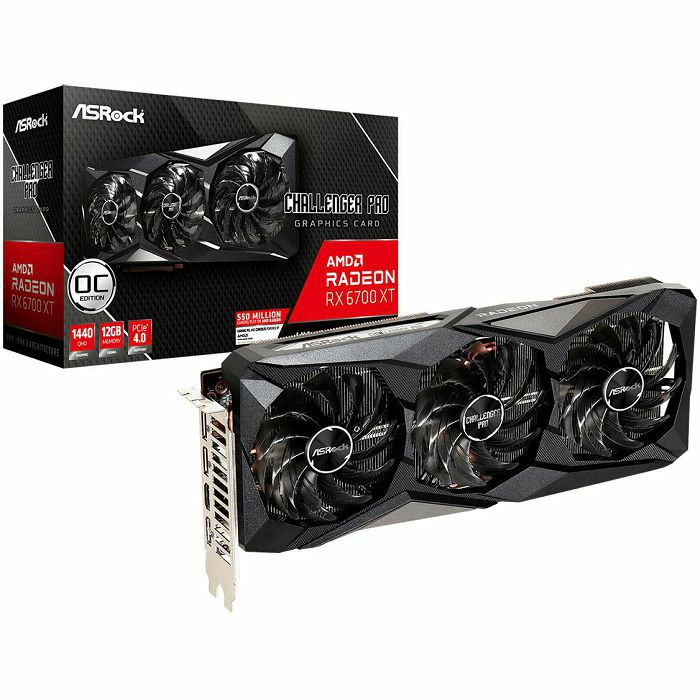
\includegraphics[scale=0.1]{Slike/graficka.jpg}
    \caption{AMD RX 6600XT}
    \label{fig:Grafička kartica}
\end{figure}
\begin{itemize}
    \item Model: AMD RX 6600XT
    \item Grafički procesor: RDNA 2
    \item Stream Processors: 2048
    \item Brzina GPU-a: Do 2589 MHz
    \item VRAM: 8GB GDDR6
    \item Sučelje: PCIe 4.0
    \item Dodatne značajke: Ray Tracing, FidelityFX Super Resolution (FSR)
    \item Obrazloženje: AMD RX 6600XT je odabran zbog izvrsnih performansi i podrške za suvremene grafičke tehnologije poput Ray Tracinga i FSR-a.
    \item Cijena: 80 EUR 
\end{itemize}
\pagebreak


\subsection{Matična ploča}
\begin{figure}[H]
    \centering
    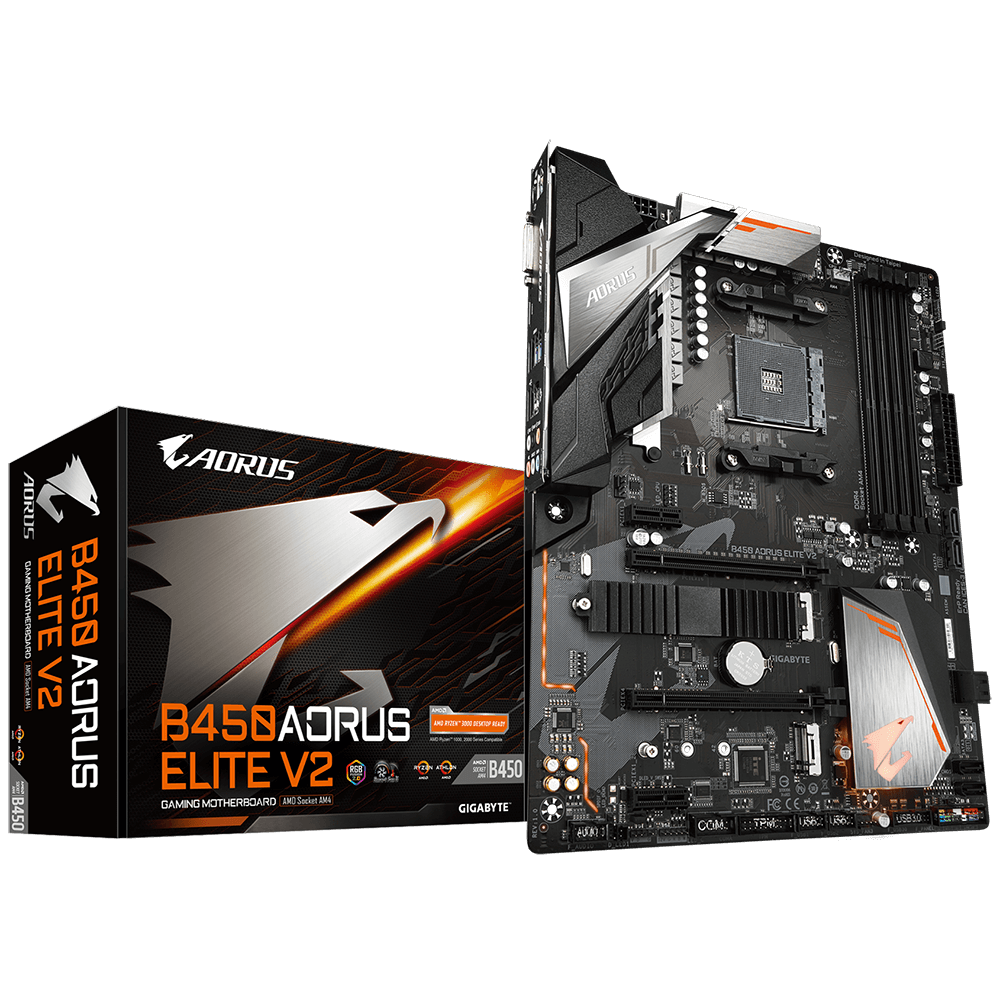
\includegraphics[scale=0.1]{Slike/Maticna.jpg}
    \caption{B450 AORUS ELITE v2}
    \label{fig:Matična}
\end{figure}
\begin{itemize}
    \item Model: B450 AORUS Elite
    \item Čipset: AMD B450
    \item Podrška za procesore: AMD Ryzen serije 3000
    \item PCIe 3.0, M.2 sučelja, USB 3.1
    \item Audio: Realtek ALC1200
    \item LAN: Intel GbE LAN
    \item Obrazloženje: B450 AORUS Elite pruža stabilnu platformu za AMD Ryzen procesore s odgovarajućim sučeljima i funkcijama potrebnim za rad s odabranim komponentama.
    \item Cijena: 130 EUR 
\end{itemize}

\subsection{RAM memorija}
\begin{figure}[H]
    \centering
    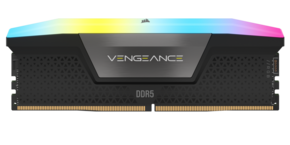
\includegraphics[scale=0.1]{Slike/ram.jpg}
    \caption{Corsair Vengeance LPX}
    \label{fig:RAM}
\end{figure}
\begin{itemize}
    \item Model: Corsair Vengeance LPX
    \item Kapacitet: 2x8GB
    \item Brzina: 3000MHz
    \item Tip: DDR4
    \item CAS Latencija: CL16
    \item Obrazloženje: Corsair Vengeance LPX pruža pouzdanu i brzu radnu memoriju koja podržava visoke performanse sustava, a odabrana je zbog ravnoteže između brzine i pouzdanosti.
    \item Cijena: 100 EUR
\end{itemize}


\subsection{Tvrdi Disk (HDD)}
\begin{figure}[H]
    \centering
    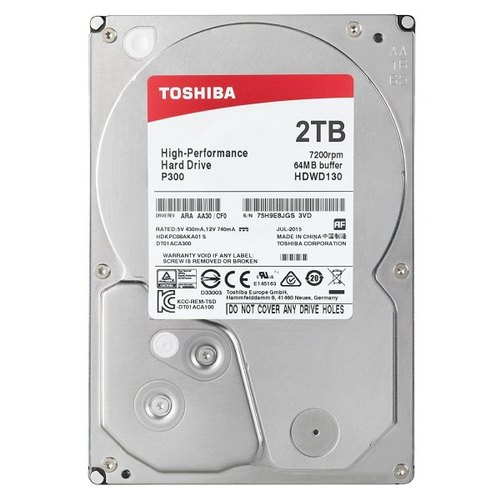
\includegraphics[scale=0.1]{Slike/HDD.jpg}
    \caption{Hard disk}
    \label{fig:HDD}
\end{figure}
\begin{itemize}
    \item Model: Toshiba 2TB HDD
    \item Kapacitet: 2TB
    \item Brzina vrtnje: 7200 RPM
    \item Cache: 64MB
    \item Sučelje: SATA3
    \item Obrazloženje: Toshiba 2TB HDD pruža dodatni prostor za pohranjivanje podataka i aplikacija koje ne zahtijevaju veliku brzinu.
    \item Cijena: 60 EUR 
\end{itemize}

\subsection{NVME ssd}
\begin{figure}[H]
    \centering
    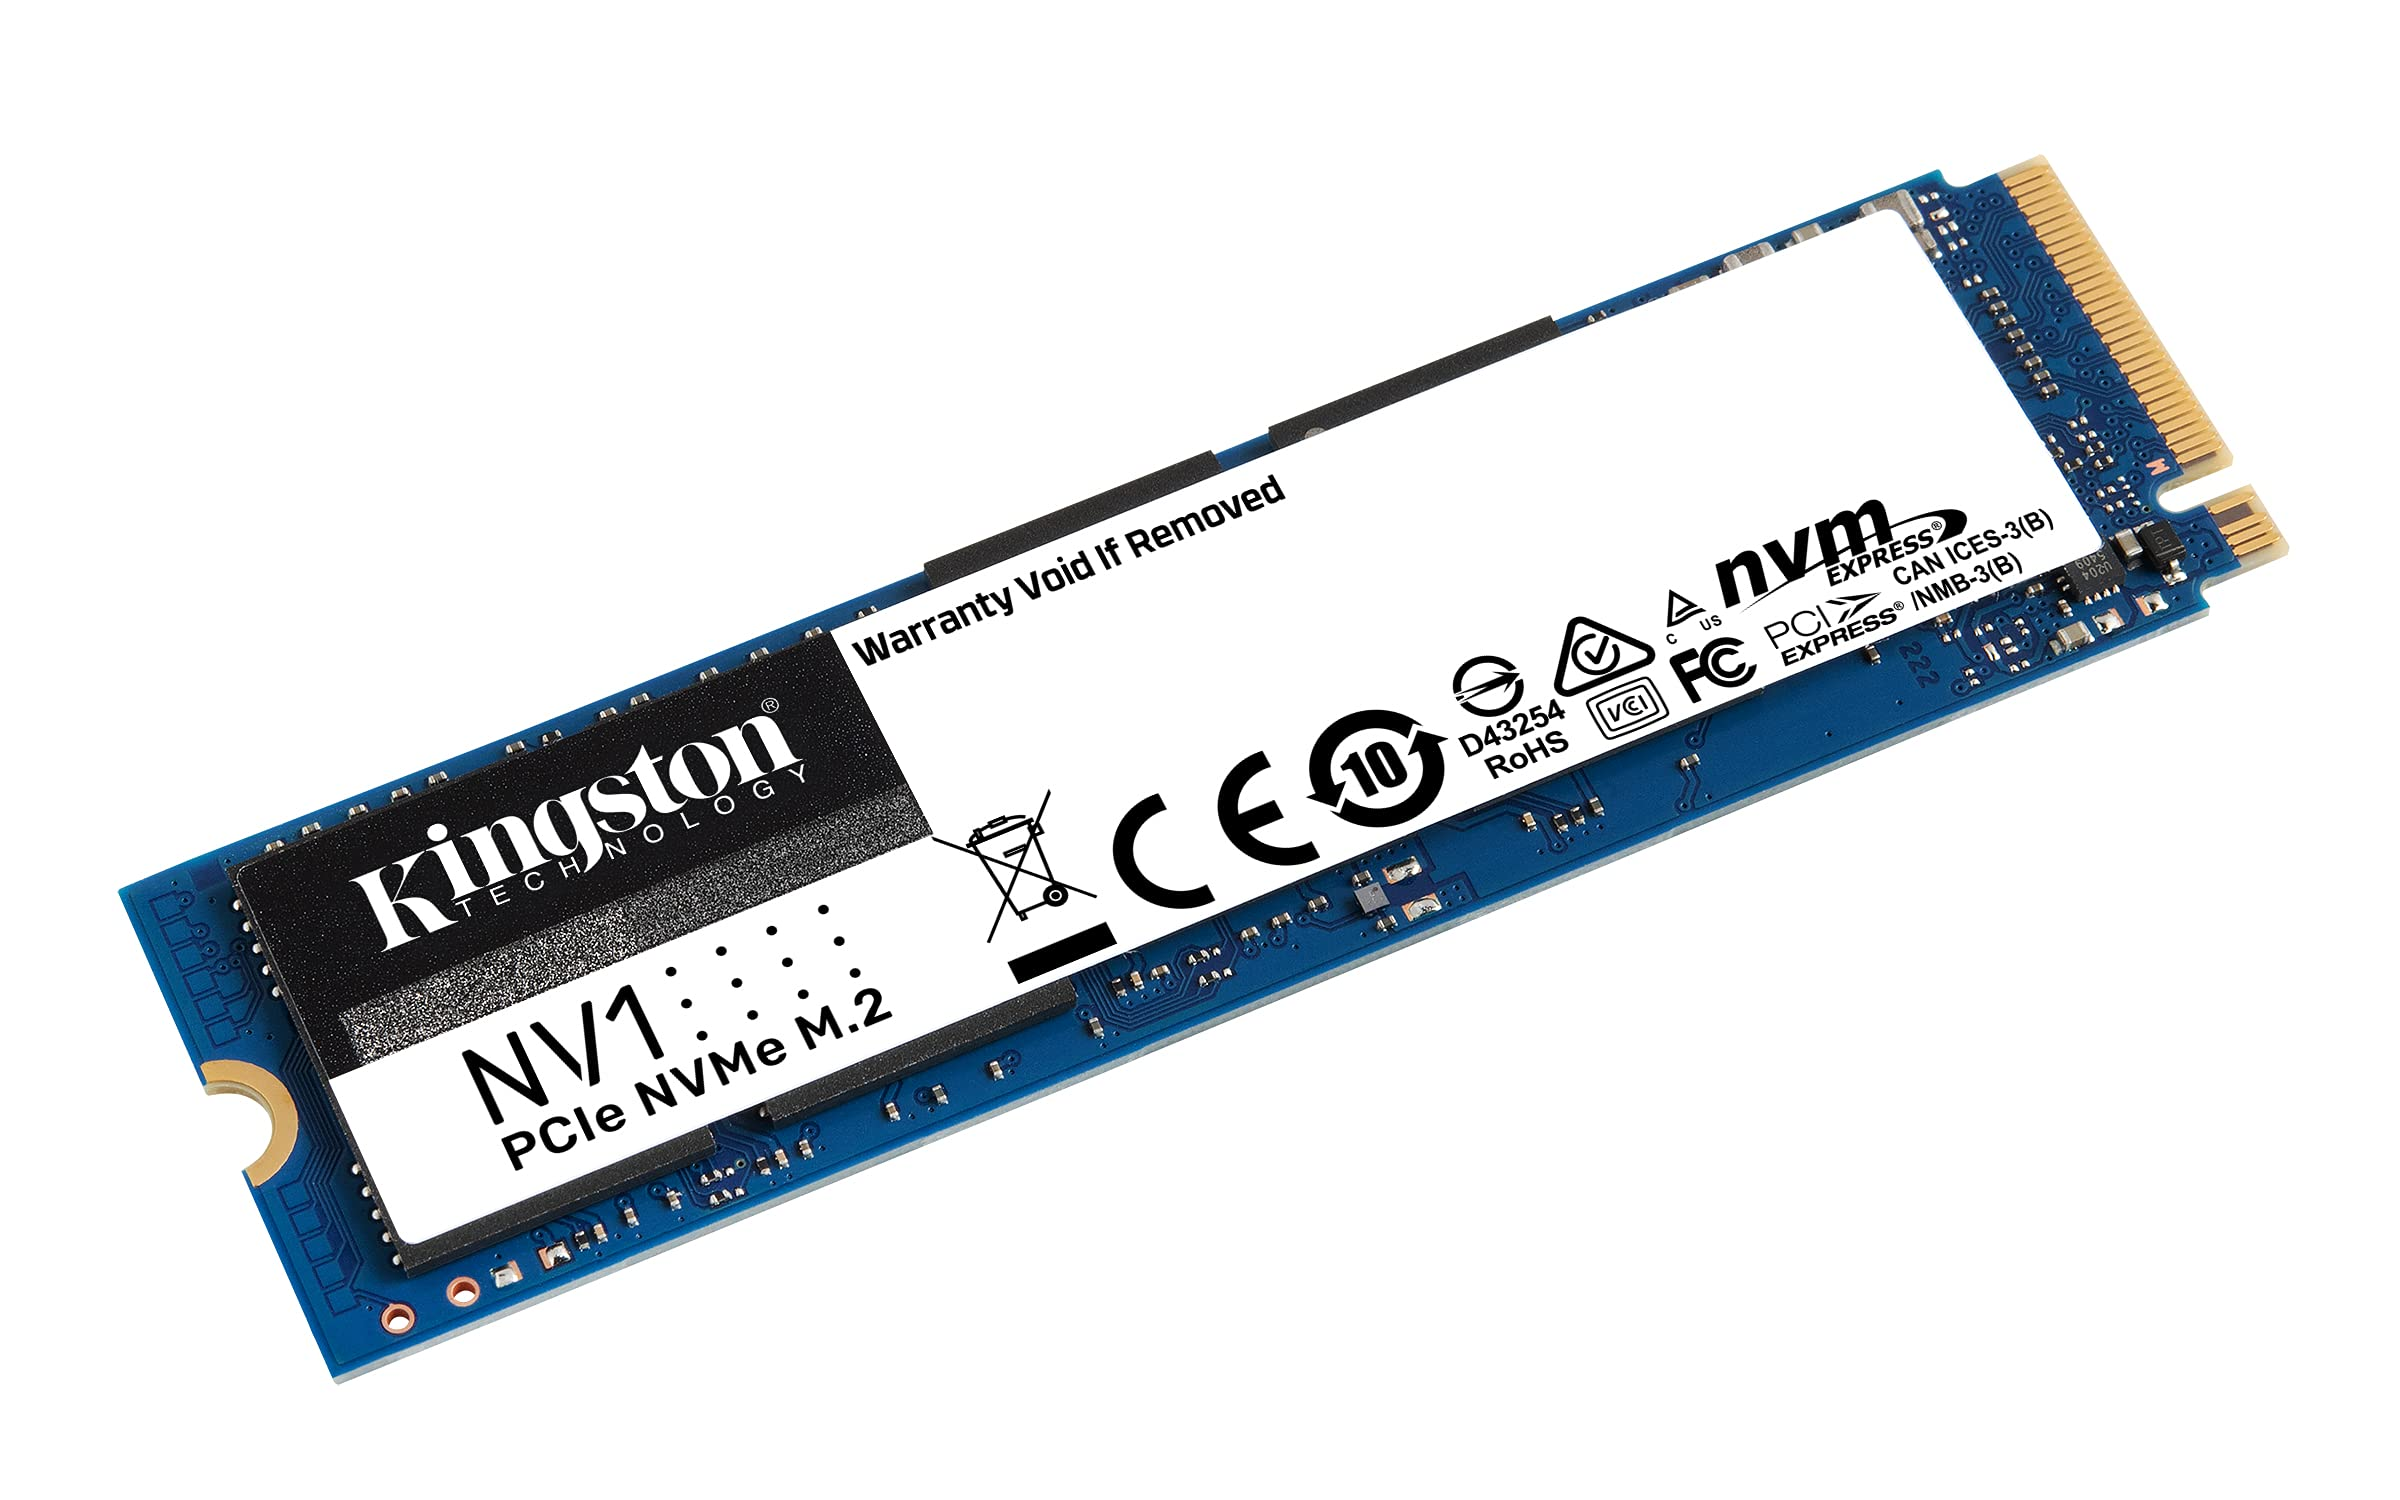
\includegraphics[scale=0.1]{Slike/NVMe.jpg}
    \caption{Kingston NV1 1TB M.2 2280 NVMe}
    \label{fig:NVMe}
\end{figure}
\begin{itemize}
    \item Model: Kingston NV1 1TB M.2 2280 NVMe
    \item Kapacitet: 1TB
    \item Sučelje: M.2 2280, NVMe
    \item Brzina čitanja: Do 2,100 MB/s
    \item Brzina pisanja: Do 1,700 MB/s
    \item Obrazloženje: Kingston NV1 1TB pruža brze prijenose podataka zahvaljujući NVMe sučelju, čineći ga odličnim izborom za brzu pohranu velikih projektnih datoteka u CAD/CAM okruženju.
    \item Cijena: 120 EUR \href{https://vacom.hr/proizvod/ssd-kingston-nv1-1tb-m-2-2280-nvme/}{Shop}
\end{itemize}

\section{Periferija}


\section{Ukupna Cijena}
\begin{itemize}
    \item lorem ipsum
\end{itemize}

\section{Zaključak}
lorem ipsum     

\end{document}
